\documentclass{templateNote}
\usepackage{tcolorbox}
\usepackage{hyperref}
\usepackage{amsmath}
\usepackage{amssymb}
\usepackage{soul}
\usepackage{circuitikz}
\usepackage{comment}
\usepackage{verbatim}


\begin{document}
\imagenlogoU{img/logoNGMFormal_sinF.png}
\linklogoU{https://github.com/NicoGomezM} 
% \imagenlogoD{img/logo-ubb-txt-face.png} 
\titulo{Apunte 1}
\asignatura{Sistemas Operativos}
\autor{
    \indent
    Nicolás {Gómez Morgado}
}


\portada
\margenes 
\tableofcontents
\newpage


\section{Importante}

\begin{itemize}
    \item Se sugiere tener instalada una distribución de Linux en el computador, en mayor medida Debian, ya que el Profesor trabaja con esta distribución.
    \item Linux y Unix están orientados al multiuser, a diferencia de Windows que esta orientado al single user.
    \item El S.O. es el intermediario entre el hardware y el usuario.
    \item Linux es el núcleo del S.O. y las distribuciones son como se adorna/agrupa este mismo.
    \item Para la tarea 1 se debe crear un programa con GNU GCC++ en Linux.
    \item Para la tarea 2 se debe crear un programa.
    \item \textbf{API:} Interfaz de programación de aplicaciones que permite a los programas comunicarse con el sistema operativo.
\end{itemize}

\newpage
\section{Introducción}
En principios de la computación no existía el software que comunicara el hardware con el usuario, por lo que se debía programar directa y físicamente en lenguaje maquina (tarjetas perforadas). La operación de estas computadoras era completamente manual.Tiempo de uso de la computadora demasiado alto, involucrando colocar tarjetas, imprimir respuestas, etc.

\subsection*{Sistemas informáticos compartidos}

Con el avance de la tecnología se separo el trabajo para operar la maquina, el operador se encargaba de insertar las tarjetas y el programador a crearlas/ordenarlas. A pesar de esta optimización la CPU seguía sin utilizarse cuando el trabajo se detenía, por lo cual se desarrollan mecanismos de secuenciamiento automático de trabajos (primeros SO).

Se implementa un monitor residente para transferir el control al trabajo siguiente. A pesar de estas mejoras aun existía tiempo muerto en la CPU debido a la diferencia de velocidades en los dispositivos de entrada/salida.

\subsection*{Sistema Batch (Lote) simple}

Los trabajos se agrupan en lotes y se ejecutan en secuencia, el monitor residente se encarga de cargar el siguiente trabajo en la memoria principal. 

\begin{figure}[H]
    \centering
    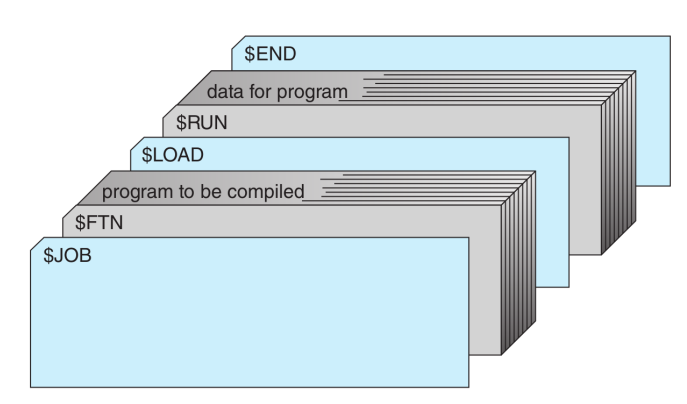
\includegraphics[width=0.5\textwidth]{img/bash_simple.png}
\end{figure}

\subsection*{E/S solapada}

Solución para reducir el tiempo muerto en la CPU, se implementa un mecanismo de E/S solapada, donde la CPU puede ejecutar otro trabajo mientras se realiza una operación de E/S ya que se guarda la información (instrucciones de las tarjetas) en las cintas magnéticas para procesarse posteriormente.

\subsection*{Spooling} Sistema de colas de trabajos, donde se almacenan los trabajos en una cola de entrada y se envían a la cola de salida para ser procesados por la CPU.

\subsection*{Que es un SO?}

\begin{itemize}
    \item Programa que actúa como intermediario entre el usuario y el hardware de la maquina cuyo propósito es proporcionar un entorno en el cual se puedan ejecutar programas de forma eficiente y controlada. 
    \item Software que gestiona el hardware.
\end{itemize}

\subsection*{Estructura de un Sistema informático}
\noindent El SO es parte del sistema general.
\begin{itemize}
    \item Hardware: Conjunto de componentes físicos que componen la computadora.
    \item Sistema Operativo
    \item Programas de aplicación
    \item Usuario: Persona, maquinas u otras computadoras que utiliza la computadora.
\end{itemize}

\noindent En ningún caso las aplicaciones que utiliza el usuario pasan directamente al hardware, por temas de seguridad y optimización. \\
Actualmente cualquier cosa que se haga en una computadoras se hace a traves del sistema operativo.


\begin{figure}[H]
    \centering
    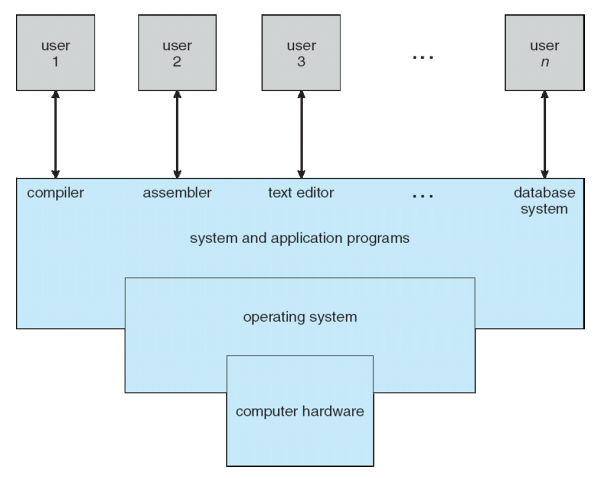
\includegraphics[width=0.5\textwidth]{img/estructura.png}
\end{figure}


\subsection*{Papel de un SO}
\begin{itemize}
    \item Punto de vista del usuario
    \begin{itemize}
        \item SO diseñado para maximizar trabajo
        \item SO diseñado para maximizar recursos
    \end{itemize}
    \item Punto de vista del sistema
    \begin{itemize}
        \item SO es un asignador de recursos
        \item SO es un Programa de control
    \end{itemize}
\end{itemize}

\begin{figure}[H]
    \centering
    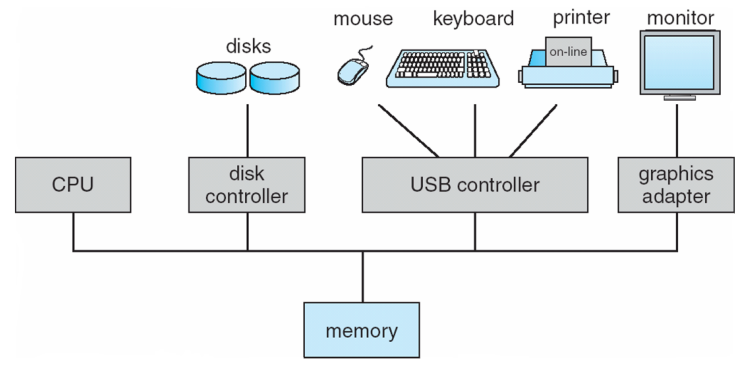
\includegraphics[width=\textwidth]{img/organizacion.png}
    \caption{Organización de un SO}
\end{figure}

\noindent\textbf{\hl{Interrupción:}} Forma que tiene el SO para enterarse de que algo ha pasado en el sistema y como reaccionar ante esto.

\subsection*{Iniciando una Computadora}
\noindent\textbf{Bootstrap:} Programa de arranque que se encuentra en la memoria ROM de la computadora, este programa se encarga de cargar el SO en la memoria RAM.
El programa de arranque se localiza y se carga el kernel a través del \textbf{GRUB} (Grand Unified Boatload) que es un gestor de arranque que permite elegir entre varios sistemas operativos.
Ante cualquier suceso inesperado, este se indica a traves de una interrupción cual puede ser de 2 formas:
\begin{itemize}
    \item Por HW: Envía señal al procesador por el BUS del sistema.
    \item Por SW: Mediante una llamada a sistema.
\end{itemize}
\noindent\textbf{Llamada a sistema:} Puente entre las aplicaciones y el SO, permite a las aplicaciones solicitar servicios al SO.
\\\\
\noindent\textbf{Controladores de dispositivos:} El hardware sabe como comunicarse con estos dispositivos de e/s gracias a estos controladores.
\\El sistema guarda los tipos de interrupciones y sus significados por lo que esa es su forma de saber como reaccionar ante estas mismas.
\\\\
\noindent\textbf{DMA:} Permite a los dispositivos de e/s acceder a la memoria sin pasar por la CPU.
\newpage
\subsection*{Almacenamiento}
\begin{enumerate}
    \item Memoria principal (RAM)
    \item Almacenamiento secundario:
    \begin{enumerate}
        \item HDD
        \item NVM
        \begin{enumerate}
            \item SSD
        \end{enumerate}
    \end{enumerate}
\end{enumerate}

\begin{figure}[H]
    \centering
    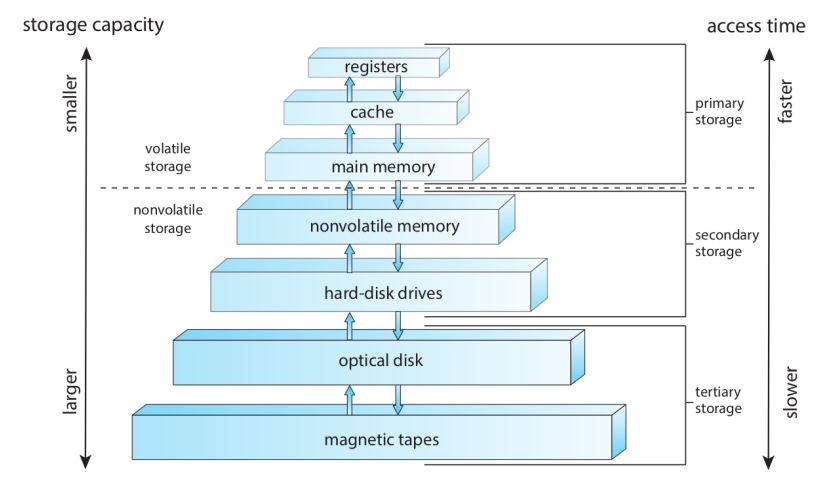
\includegraphics[width=\textwidth]{img/almacenamiento.png}
\end{figure}

\subsection*{Caching}
Información es copiada desde almacenamientos lentos a almacenamientos rápidos para mejorar la velocidad de acceso a la información.

\subsection*{Sistema multiprocessor}
Dos o mas procesadores que comparten el bus del computador, estos procesadores pueden compartir la memoria y los dispositivos de e/s.

\subsection*{Sistemas NUMA (Non-Uniform Memory Access)}
Division no uniforme de acceso a la memoria. Rápido cuando CPU necesita acceder a su memoria. Latencia aumenta si necesita acceder a memoria remota.

\subsection*{Cluster}
Varios nodos donde cada uno puede tener uno o varios procesadores. Comparten almacenamiento a través de areas de almacenamiento ( SAN - Storage Area Network).
\begin{itemize}
    \item Asimétrico: Sistema en modo de espera y monitorea a la activa.
    \item Simétrico: Todos los sistemas activos y se monitorear entre significados
\end{itemize}

\subsection*{Multiprogramación}
Organiza los trabajos para que la CPU no este ociosa, se ejecutan varios trabajos a la vez. CUando el trabajo en ejecución tiene que esperar el sistema cambia a otro trabajo.

\subsection*{Tiempo compartido}
Asigna tiempos (menos de 1 seg) entre tareas de manera equitativa, conmutando entre programas. Si los procesos no encajan en la memoria, con el swapping se pueden mover a la memoria secundaria.
\\\\
\noindent\textbf{Swapping:} Mecanismo que permite mover procesos entre la memoria principal y la secundaria.

\subsection*{Operación en Modo Dual}
Se necesitan 2 modos de operación para proteger el SO y los programas de usuario. Estos son el modo \textbf{usuario} y el modo \textbf{kernel}.

\subsection*{Temporizador}
Se asegura el control del SO sobre la CPU, se impide que los programas entren en ciclos infinitos, se impide acapararon de recursos, se usan contadores que después de un tiempo determinado generan una interrupción.

\subsection*{Gestión de procesos}
Proceso es programa en ejecución, unidad de trabajo de un SO. Programa = entidad pasiva, proceso = entidad activa. Estos procesos necesitan recursos para completar su tarea:
\begin{itemize}
    \item CPU
    \item Memoria
    \item E/S
    \item Datos de entrada
\end{itemize}

\newpage
\section{Estructuras de un SO}

\subsection*{Servicios del SO}
Un SO proporciona servicios a los programas de aplicación y a los usuarios, estos servicios pueden ser:
\begin{itemize}
    \item Interfaz de usuario: Interfaz gráfica o de línea de comandos.
    \item Ejecución de programas: Carga de programas en memoria y ejecución.
    \item Operaciones de E/S: Operaciones de lectura y escritura.
    \item Manipulación de sistema de archivos: Creación, eliminación, copia, etc.
    \item Comunicaciones: Comunicación entre procesos. Mediante:
    \begin{itemize}
        \item Memoria compartida.
        \item Paso de mensajes.
    \end{itemize}
    \item Detección de errores: Errores de hardware y software.
    \begin{itemize}
        \item Detección en HW de CPU y memoria por fallos de alimentación, en dispositivos de E/S por fallos de conexión, etc.
        \item Por cada error el SO debe decidir que hacer.
        \item La depuración ayuda a encontrar errores en el software. 
    \end{itemize}
\end{itemize}
\noindent Mas funciones centradas en garantizar la eficiencia del sistema pueden ser:
\begin{itemize}
    \item Asignación de recursos: CPU, memoria, dispositivos de E/S.
    \item Contabilidad: Uso de recursos.
    \item Protección y seguridad: Control sobre el uso de la información.
    \begin{itemize}
        \item Protección: Asegurar que todos los accesos a los recursos sean legales.
        \item Seguridad: Proteger el sistema de accesos no autorizados.
    \end{itemize}
\end{itemize}

\begin{figure}[H]
    \centering
    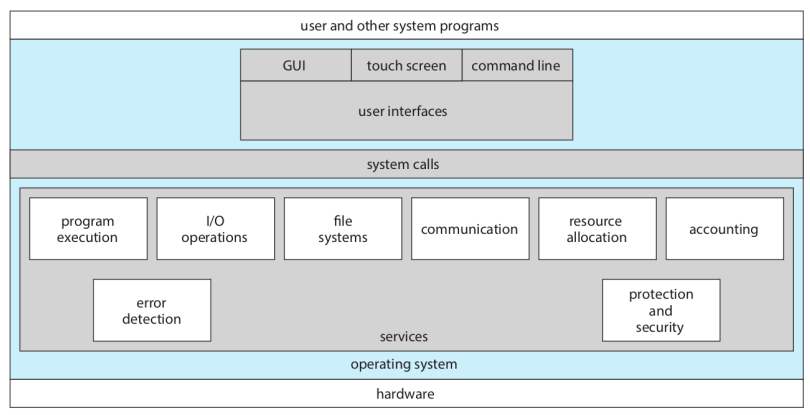
\includegraphics[width=0.8\textwidth]{img/servicios.png}
\end{figure}

\subsection*{CLI}
Interfaz de línea de comandos, permite al usuario comunicarse con el SO mediante comandos. La función principal es obtener y ejecutar los comandos del usuario.

\subsection*{GUI}
Interfaz gráfica de usuario, permite al usuario comunicarse con el SO mediante ventanas, iconos, menús, etc. La función principal es obtener y ejecutar los comandos del usuario.

\subsection*{Touchscreen}
Interfaz táctil, permite al usuario comunicarse con el SO mediante la pantalla táctil. La función principal es obtener y ejecutar los comandos del usuario.

\subsection*{Llamadas a sistema}
Proporciona una interfaz entre el SO y los programas de aplicación, permite a los programas solicitar servicios al SO. Se utiliza la API para tener el conjunto de funciones que se pueden utilizar.

\subsection*{Implementación de llamadas a sistema}
Cada llamada a sistema tiene un número asociado, el cual se almacena en un registro y se ejecuta una instrucción de interrupción. El SO tiene una tabla de interrupciones que contiene las direcciones de memoria de las rutinas de servicio.

\subsection*{Tipos de llamadas a sistema}

\begin{itemize}
    \item Control de procesos: Creación, terminación, suspensión, etc.
    \item Manipulación de archivos: Creación, eliminación, apertura, cierre, etc.
    \item Manipulación de dispositivos: Lectura, escritura, apertura, cierre, etc.
    \item Mantenimiento de información: Obtener información del sistema, configuración, etc.
    \item Comunicaciones: Creación, eliminación, envío, recepción, etc.
\end{itemize}

\subsection*{Programas del sistema}

Proporcionan un entorno cómodo para desarrollar y ejecutar programas:
\begin{itemize}
    \item Administrador de archivos: Creación, eliminación, copia, etc. 
    \item Información de estado: Información sobre cosas sencillas (hora) y complejas (rendimiento).
    \item Modificación de archivos: Edición de archivos.
    \item Soportes de lenguaje: Compiladores, ensambladores, etc.
    \item Carga y ejecución de programas: Carga de programas en memoria y ejecución.
    \item Comunicaciones: Mecanismos para crear conexiones virtuales entre procesos, usuarios y computadoras.
\end{itemize}

\subsection*{Diseño e implementación de un SO}

Métodos adecuados para el diseño e implementación de un SO:

\begin{itemize}
    \item Objetivos de diseño: definir los objetivos del sistema.
    \begin{itemize}
        \item Elegir HW.
        \item Tipo de sistema (por lotes, tiempo compartido, etc).
        \item Objetivos del usuario (comodidad, facilidad, etc) y de sistema (facilidad de diseñar, implementar, mantener, etc).
    \end{itemize}
    \item Mecanismos (como hacer algo) e implementación de políticas (que hacer).
    \begin{itemize}
        \item Ejemplo: El temporizador es un mecanismo para controlar la CPU, la política es que cada proceso tiene un tiempo limitado de ejecución.
        \item Separación de mecanismos y políticas: Los mecanismos deben ser generales y las políticas específicas. Permite la flexibilidad para el cambio futuro de las políticas.
    \end{itemize}
    \item Implementación
    \begin{itemize}
        \item Completado el diseño debe implementarse, tradicionalmente en ensamblador, pero hoy en dia se utiliza C y C++.
    \end{itemize}
\end{itemize}

\subsection*{Estructura de un SO}

La ingeniería de un SO debe hacerse de tal forma que sea fácil de modificar y funcione de la manera esperada. Un método habitual para lograr estos puntos es dividir en componentes mas pequeños en lugar de un sistema monolítico(estructura modular).
Cada uno de los componentes deben definirse bien con E/S y sus funciones especificadas.

\subsubsection*{Estructura simple}
\begin{itemize}
    \item No existe protección ni multiprogramación.
    \item Falla en la programación puede encadenar una caída en el sistema.
    \item MS-DOS (Microsoft Disk Operating System) diseñado para maxima funcionalidad en el menor espacio posible.
    \item MS-DOS diseñado en HW no daba soporte protección ni modo dual.
\end{itemize}

\begin{figure}[H]
    \centering
    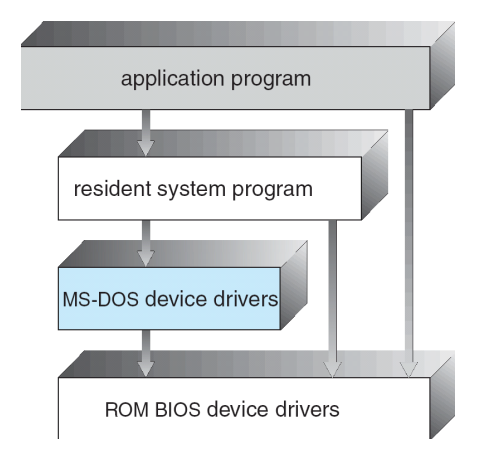
\includegraphics[width=0.5\textwidth]{img/estSim.png}
\end{figure}

\subsubsection*{Sistema monolíticos}
\begin{itemize}
    \item Permiten multiprogramación y multiples usuarios.
    \item SO es conjunto de procedimientos que se agrupan en el núcleo.
    \item Núcleo protegido (modo dual).
    \item Núcleo de gran tamaño, no modular.
    \item Ante cualquier cambio se compila el núcleo por completo
\end{itemize}

\begin{figure}[H]
    \centering
    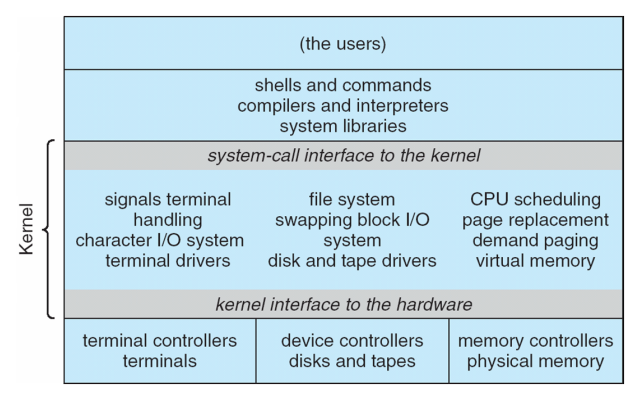
\includegraphics[width=0.5\textwidth]{img/estMono.png}
\end{figure}

\subsubsection*{Estructura en niveles}
\begin{itemize}
    \item Mejor modularización y protección de los componentes del sistema.
    \item Oculta detalles a niveles superiores, dando a los programadores mas libertad para la implementación de rutinas de bajo nivel.
    \item Comunicación entre niveles significa mucho costo de operación (Overhead).
    \item Se hace difícil definir bien los niveles ya que cada nivel usa servicios del nivel inferior.
\end{itemize}

\begin{figure}[H]
    \centering
    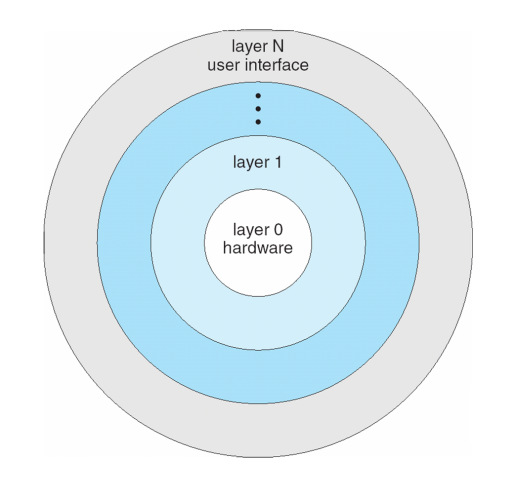
\includegraphics[width=0.4\textwidth]{img/estNiv.png}
\end{figure}

\subsubsection*{Microkernel}
\begin{itemize}
    \item Quita componentes no esenciales del kernel y los implementa como programas de sistema y de nivel usuario.
    \item Kernel mas pequeño y fácil de mantener.
    \item Facilidad ampliación SO (se añaden los servicios nuevos al espacio del usuario sin tener que modificar el kernel).
    \item Pueden presentar peor rendimiento en comparación a otras estructuras debido a la carga adicional de procesamiento.
    \item Primeras versiones: Windows NT, QNX, Mach, Chorus, etc.
\end{itemize}

\subsubsection*{Módulos}
\begin{itemize}
    \item Implementados en los SSOO mas modernos.
    \item Kernel dispone componentes fundamentales.
    \item Enlaza de forma dinámica los módulos (servicios adicionales) en tiempo de ejecución.
    \item Versiones mas conocidas: Solaris, Linus, Mac OS X, etc.
\end{itemize}

\begin{figure}[H]
    \centering
    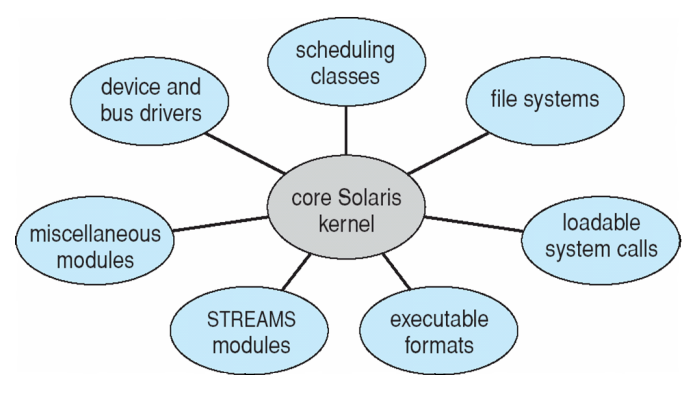
\includegraphics[width=0.5\textwidth]{img/estMod.png}
\end{figure}

\subsubsection*{Máquinas virtuales}
\begin{itemize}
    \item Emula una computadora física.
    \item Permite ejecutar varios sistemas operativos en una misma maquina.
    \item Se implementa en el nivel de usuario.
    \item Permite compartir un mismo HW en diferentes sistemas operativos de forma concurrente.
    \item Ejemplos: Java, .NET, etc.
\end{itemize}

\begin{figure}[H]
    \centering
    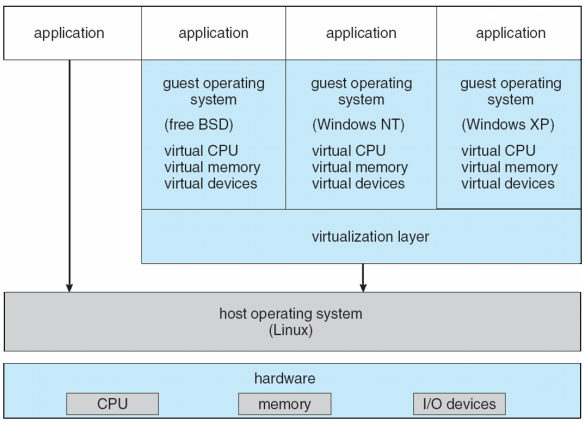
\includegraphics[width=0.8\textwidth]{img/estMaq.png}
\end{figure}

\newpage
\section*{Procesos}

\subsection*{Concepto de proceso}
\begin{itemize}
    \item Programa en ejecución.
    \item Unidad de trabajo del SO.
    \item Entidad activa.
    \item Proceso = Programa + Estado del proceso.
\end{itemize}
Ademas del código un proceso también tiene:
\begin{enumerate}
    \item \textbf{Contador de programa}: Indica la siguiente actividad actual.
    \item \textbf{Pila-Stack}: Almacena las llamadas a subrutinas y las variables locales (datos temporales).
    \item \textbf{Sección de datos}: Contiene variables globales.
\end{enumerate}

\subsection*{Estructura de un proceso en memoria}
\begin{figure}[H]
    \centering
    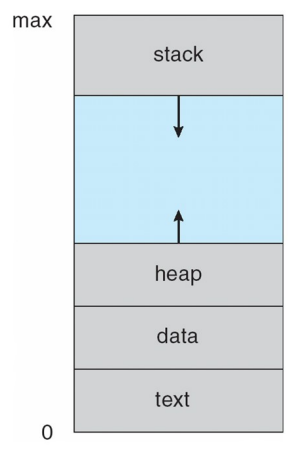
\includegraphics[width=0.5\textwidth]{img/estProceso.png}

    Text = Código programa \\
    Heap = Memoria global y reservada
\end{figure}

\subsection*{Estado del proceso}
\begin{enumerate}
    \item \textbf{Nuevo}: Proceso esta siendo creado.
    \item \textbf{En ejecución}: Instrucciones se están ejecutando.
    \item \textbf{En espera}: Proceso espera por un evento (terminación operación E/S, recepción de una señal, etc.).
    \item \textbf{Preparado (Listo)}: Proceso espera por la CPU.
    \item \textbf{Terminado}: Proceso ha terminado de ejecutarse.
\end{enumerate}
\begin{figure}[H]
    \centering
    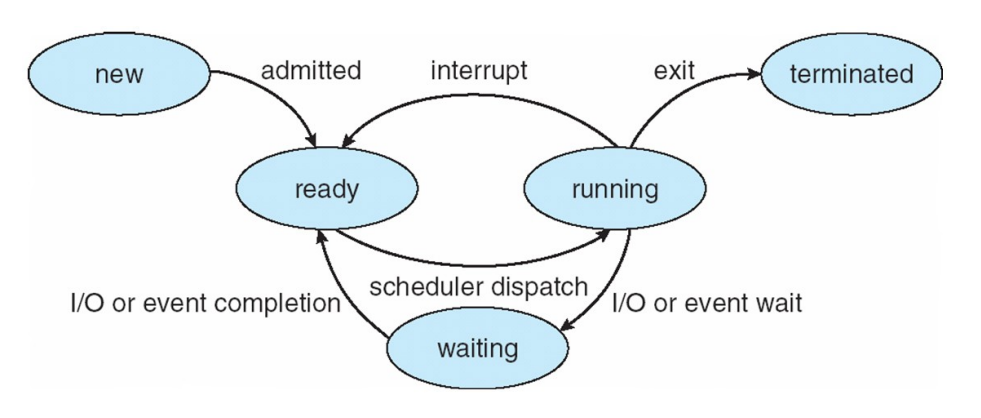
\includegraphics[width=\textwidth]{img/estadosProceso.png}
    \caption{Hormiga de estados de un proceso}
    \label{fig:hormiga-estados}
\end{figure}

\subsection*{Bloque de control de procesos}
Cada proceso se representa en el SO mediante un bloque de control de procesos (\textbf{PCB: process control block}), este contiene toda la información necesaria para la gestión del proceso. La información contenida en el PCB es:
\begin{itemize}
    \item Estado del proceso: Nuevo, listo, en ejecución, en espera, terminado, etc.
    \item Contador de programa: Dirección de la próxima instrucción a ejecutar.
    \item Registros de la CPU: Contenido de los registros de la CPU (acumulador, contador de instrucciones, etc).
    \item Información de planificación de la CPU: Prioridad del proceso, tiempo de ejecución, etc.
    \item Información de gestión de memoria: Información sobre la memoria asignada al proceso (valores de los registros base y límite, tablas de segmentos o paginas, etc.).
    \item Información contable: Tiempo de CPU utilizado, numero del proceso, tiempo de reloj real, tiempo de CPU en espera, etc.
    \item Información del estado E/S: Lista de dispositivos E/S asignados al proceso, estado de los dispositivos, etc.
\end{itemize}

\begin{figure}[H]
    \centering
    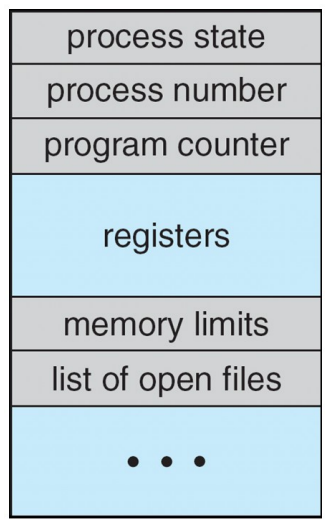
\includegraphics[width=0.25\textwidth]{img/pcb.png}
\end{figure}

\subsection*{Planificación de procesos}
El objetivo de la \textbf{multiprogramación} el lograr maximizar la utilización de la CPU ejecutando varios procesos simultáneamente. 

El objetivo del \textbf{tiempo compartido} es conmutar (cambiar) la CPU entre varios procesos con una frecuencia tan alta que los usuarios puedan interactuar con cada programa mientras se ejecuta.

Para lograr el cumplimiento de estos objetivos la planificación de procesos se encarga de seleccionar el proceso que se ejecutara en la CPU en un momento dado.

\subsection*{Colas de planificación}
Apenas los procesos llegan al sistema se colocan en Cola de trabajos la cual se encarga de almacenar todos los procesos que llegan al sistema. Dentro de esta cola se pueden encontrar varias colas de planificación:
\begin{itemize}
    \item \textbf{Cola de procesos preparados (listos)}: Procesos almacenados en memoria principal y listos para ser ejecutados.
    \item \textbf{Cola de espera}: Procesos que están esperando por un evento (E/S, señal, etc).    
\end{itemize}

Estas colas se almacenan en forma de listas enlazadas donde la cabeza de la cola apunta al primer y al ultimo PCB. 

\begin{figure}[H]
    \centering
    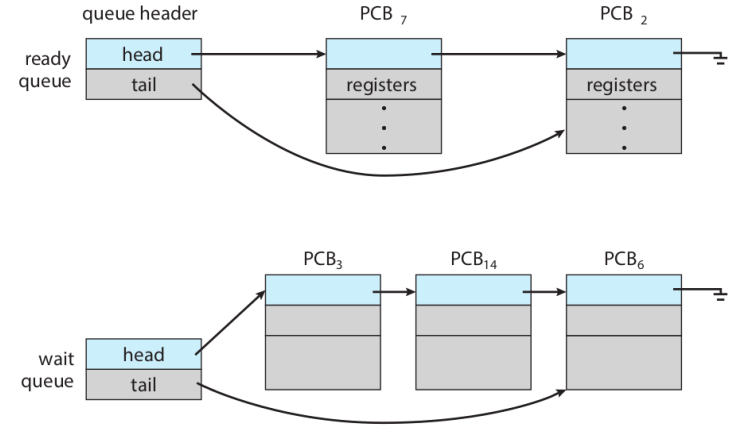
\includegraphics[width=\textwidth]{img/colas.png}
    \caption{Colas de procesos listos y en espera}
\end{figure}

\subsection*{Diagrama de colas}
A continuación se presentara una representación que explica la planificación de procesos en un SO. Dentro de esta representación se van a encontrar 2 tipos de colas, la cola de procesos listos y la cola de procesos en espera.
Los círculos representan los recursos que le dan servicios a las colas y las flechas el flujo que sigue el proceso en el sistema.

\begin{figure}[H]
    \centering
    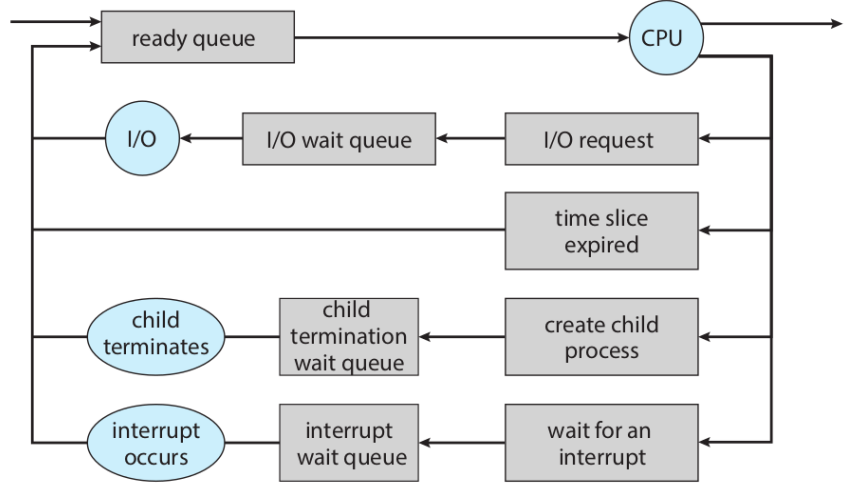
\includegraphics[width=0.8\textwidth]{img/diagr.png}
\end{figure}

\newpage
\subsection*{Planificación de CPU}
Para entender lo que hace la planificación de CPU se debe entender que los procesos se mueven entre diversas colas durante su ciclo de vida, por lo que es imperante una planificación.
El planificador de CPU selecciona un proceso de la cola de procesos listos y lo asigna a la CPU. Esta selección de proceso es muy frecuente ya que normalmente se hace cada 100 ms o menos.

\subsubsection*{Planificación intermedia - Swapping}
Algunos SSOO presentan este tipo de planificación, el cual se basa en un \textbf{intercambio}, donde el planificador descarga un proceso (swap out) de la memoria principal a la secundaria y carga otro proceso (swap in) de la memoria secundaria a la principal.
Esta planificación logra reducir el grado de la multiprogramación, mejora la mezcla de procesos, libera memoria, etc.

\begin{figure}[H]
    \centering
    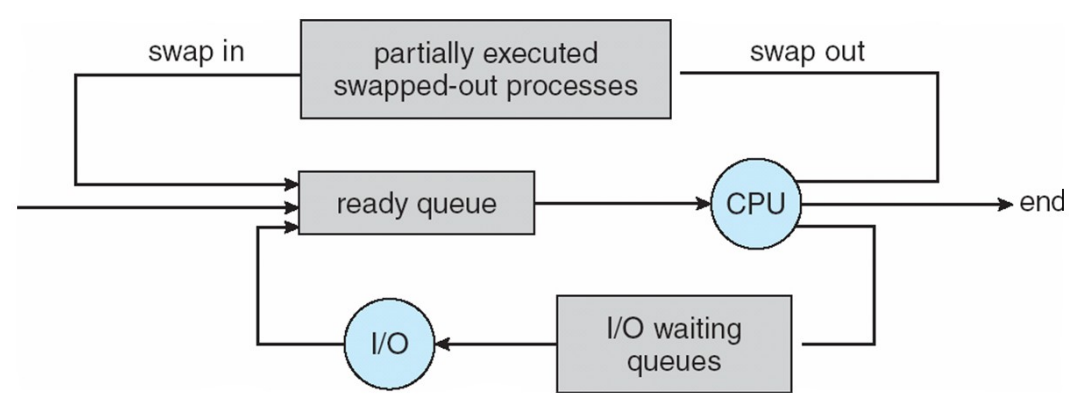
\includegraphics[width=0.5\textwidth]{img/swapping.png}
\end{figure}

\subsection*{Cambios de contexto}
Es una interrupción que provoca que el SO obligue a la CPU a abandonar su tarea actual para ejecutar una rutina del kernel. 
Cuando se realiza este cambio de contexto el mismo evento debe encargarse de guardar el estado del proceso que va a ser interrumpido y cargar el estado del proceso que va a ser ejecutado.
Estos contextos se almacenan en el PCB de cada proceso. Se debe tener en consideración que el tiempo utilizado en el cambio de contexto es tiempo muerto.

\begin{figure}[H]
    \centering
    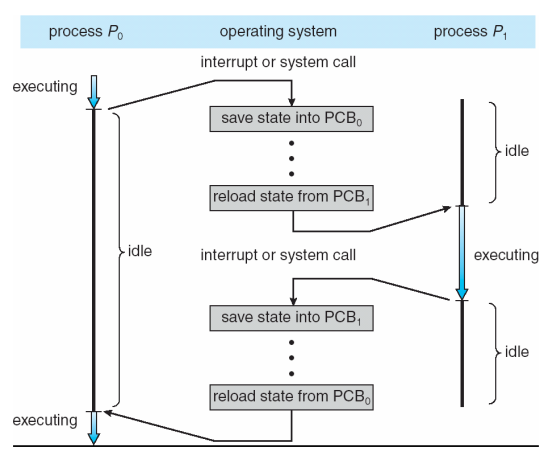
\includegraphics[width=0.5\textwidth]{img/cambioCont.png}
\end{figure}


\subsection*{Operaciones sobre los procesos}
La \textbf{creación} y \textbf{eliminación} de procesos debe estar respaldada por mecanismos adecuados, ya que, en la mayoría de los sistemas, los procesos se ejecutan de forma concurrente y se gestionan de manera dinámica.

\subsubsection*{Creación de procesos}
Mientras se ejecuta un proceso, este mismo puede crear uno o varios procesos adicionales a traves de las llamadas a sistema \textbf{fork()} o \textbf{exec()}. Algunas características de la creación de procesos son:
\begin{itemize}
    \item Proceso creador se conoce como \textbf{proceso padre}.
    \item Procesos creados se conocen como \textbf{procesos hijos}.
    \item Procesos hijos pueden a su vez crear otros procesos (árbol de procesos).
    \item Cada proceso, ya sea hijo o padre, presenta un identificador único (pid, process identifier).
    \item Ya se sabe que un proceso necesita de recursos para funcionar, por lo que cuando un proceso crea otro, este nuevo puede:
    \begin{itemize}
        \item Obtener recursos propios.
        \item Obtener subconjunto de recursos del proceso padre.
    \end{itemize}
    \item Al crear un proceso hijo, existen 2 posibilidades de ejecución:
    \begin{itemize}
        \item El padre se ejecuta concurrentemente con el hijo.
        \item El padre espera a que el/los hijo/s terminen de ejecutarse a traves de la llamada a sistema \texttt{wait()}.
    \end{itemize}
    \item Existen 2 posibilidades en función del espacio de direcciones del proceso hijo:
    \begin{itemize}
        \item Hijo es una copia exacta del padre (mismos datos, variables, etc).
        \item Hijo es un programa completamente nuevo.
    \end{itemize}
    \item Para UNIX:
    \begin{itemize}
        \item Llamada a sistema \texttt{fork()} crea un nuevo proceso.
        \item Llamada a sistema \texttt{exec()} se utiliza después del \texttt{fork()} y se encarga de reemplazar el espacio de direcciones del proceso actual con un nuevo programa.
    \end{itemize}
\end{itemize}

\begin{figure}[H]
    \centering
    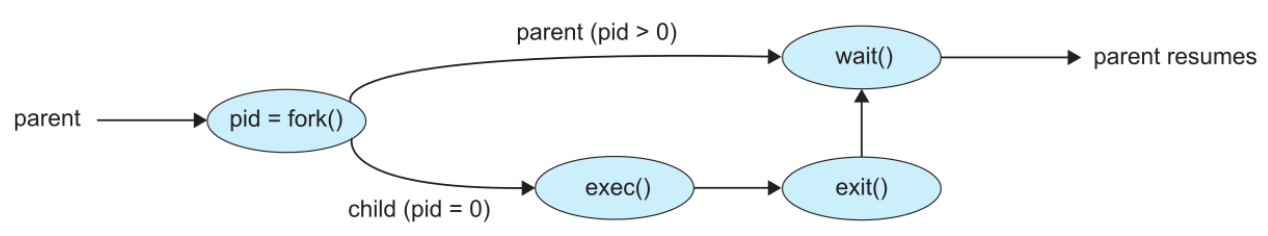
\includegraphics[width=\textwidth]{img/creacion.png}
\end{figure}


\subsubsection*{Eliminación de procesos}

Un proceso se elimina cuando ha terminado de ejecutarse, ya sea por finalización normal o por error, y pide al SO que lo elimine a traves de la llamada a sistema \texttt{exit()}. Algunas características de la eliminación de procesos son:
\begin{itemize}
    \item Proceso hijo puede devolver su estado al padre mediante \texttt{wait(\&status)}.
    \item SO libera los recursos de un proceso eliminado.
    \item Proceso padre puede eliminar a un proceso hijo por las siguientes razones:
    \begin{itemize}
        \item Hijo excede los recursos permitidos.
        \item Tarea del hijo ya no es necesaria.
        \item Padre abandona el sistema, el SO no permite la ejecución de procesos huérfanos.
    \end{itemize}
\end{itemize}

\subsection*{Comunicaron interprocesos}
Los procesos que se ejecutan concurrentemente pueden ser:
\begin{itemize}
    \item \textbf{Independientes}: No comparten datos.
    \item \textbf{Cooperativos}: Comparten datos.
\end{itemize}

El permitir la cooperación entre procesos puede ser beneficioso, ya que:
\begin{itemize}
    \item Permite a los procesos cooperar en la realización de una tarea.
    \item Permite a los procesos compartir datos (varios usuarios pueden acceder a la misma data).
    \item Permite a los procesos comunicarse.
    \item Acelera cálculos y divide tareas.
    \item Ejecución en paralelo (varias CPU's).
    \item Permite la construcción de sistemas modulares (modularidad), dividiendo las funciones del sistema en diferentes procesos.
\end{itemize}

La cooperación entre procesos necesita de mecanismos de comunicación (IPC, Interprocess Communication) que permitan a los procesos compartir datos y sincronizar sus actividades. Existen 2 tipos de modelos de IPC:
\begin{itemize}
    \item \textbf{Modelo de memoria compartida}: 
    \begin{itemize}
        \item Region en memoria la cual es compartida por varios procesos cooperativos.
        \item Intercambio de información entre procesos escribiendo/leyendo en la región de memoria compartida.
        \item Permite velocidades máximas (velocidad de memoria).
    \end{itemize}
    \newpage
    \item \textbf{Modelo de paso de mensajes}:
    \begin{itemize}
        \item Comunicación mediante intercambio de mensajes.
        \item Mas complejidad en la implementación.
        \item Menor velocidad ya que usa llamadas al sistema, teniendo que intervenir el kernel.
    \end{itemize}
\end{itemize}

\begin{figure}[H]
    \centering
    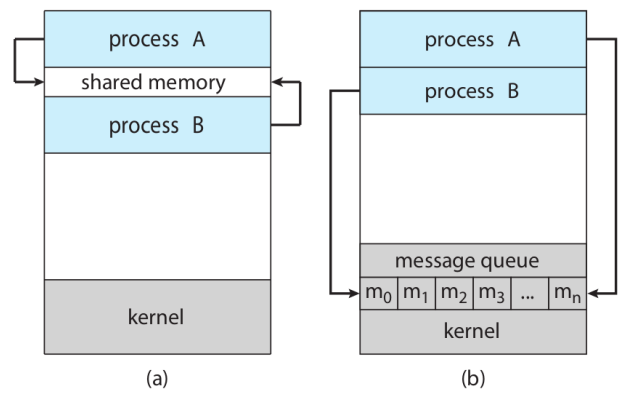
\includegraphics[width=0.8\textwidth]{img/ipc.png}

    (a) Memoria compartida \hspace{1.5cm} (b) Paso de mensajes
\end{figure}

\subsubsection*{Memoria compartida -> API's}

Para hacer uso de la memoria compartida se pueden/deben utilizar las siguientes API's:
\begin{itemize}
    \item IEEE POSIX Threads (PThreads):
    \begin{itemize}
        \item Standard Unix threading API (Windows)
        \item Más de 60 funciones: pthread create, pthread join, pthread exit, etc.
        \item Bajo nivel.
        \item Manejo explicito de hebras (creación, terminación, sincronización, etc).
    \end{itemize}
    \item OpenMP:
    \begin{itemize}
        \item API de programación en paralelo.
        \item Directivas de compilador.
        \item API de funciones.
        \item Alto nivel de abstracción.
        \item Manejo implícito de hebras.
        \item Disponible para C, C++, Fortran.
        \item Énfasis HPC (High Performance Computing).
    \end{itemize}
\end{itemize}

\subsubsection*{Paso de mensajes -> API's}
Se observan varios procesos ejecutándose en diferentes nodos, de los cuales cada proceso tiene su espacio de direcciones privado.
El acceso de los datos se realiza de forma remota mediante envió/recepción de mensajes, donde MPI (Message Passing Interface) es la API más utilizada para la programación de paso de mensajes.

\subsection*{Sockets}
Los mecanismos de comunicación vistos anteriormente son utilizados para la comunicación entre procesos en la misma máquina. Para la comunicación entre procesos en diferentes máquinas se utilizan los sockets.
Los sockets son un mecanismo de comunicación que permite la comunicación entre procesos en diferentes máquinas a través de la red. Los sockets son utilizados en la programación de redes y permiten la comunicación entre procesos en diferentes máquinas.
La forma de utilización de sockets se puede resumir en los siguientes pasos:
\begin{itemize}
    \item Par de procesos emplean una pareja de sockets para establecer comunicación.
    \item Se identifican por una dirección IP y un número de puerto.
    \item Servidores implementan servicios que \textbf{escuchan} en un puerto conocido (80->HTTP, 21->FTP, etc).
    \item Cliente X \texttt{146.86.5.20:1625} tiene establecida una conexión con el servidor web: \texttt{161.25.19.8:80} 
\end{itemize}

\begin{figure}[H]
    \centering
    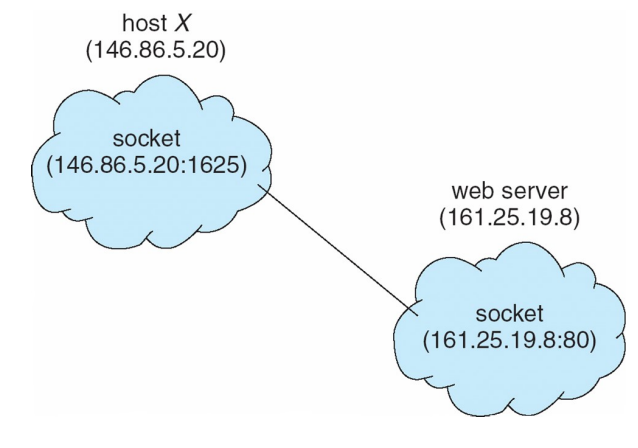
\includegraphics[width=0.5\textwidth]{img/sockets.png}
\end{figure}

\newpage
\section{Hebras (Threads)}
Las hebras son la unidad básica de utilización de la CPU. Estas comprenden:
\begin{itemize}
    \item ID de la hebra.
    \item Contador de programa.
    \item Conjuntos y registros de pila.
\end{itemize}
Y comparte con otras hebras:
\begin{itemize}
    \item Sección de código.
    \item Sección de datos.
    \item Otros recursos del SO.
\end{itemize}
Un proceso tradicional comprende solo una hebra de control, osea \textbf{monohebra (single-threaded)}. 
De igual manera un proceso con múltiples hebras se conoce como proceso \textbf{multihebras (multithreaded)}.

\begin{figure}[H]
    \centering
    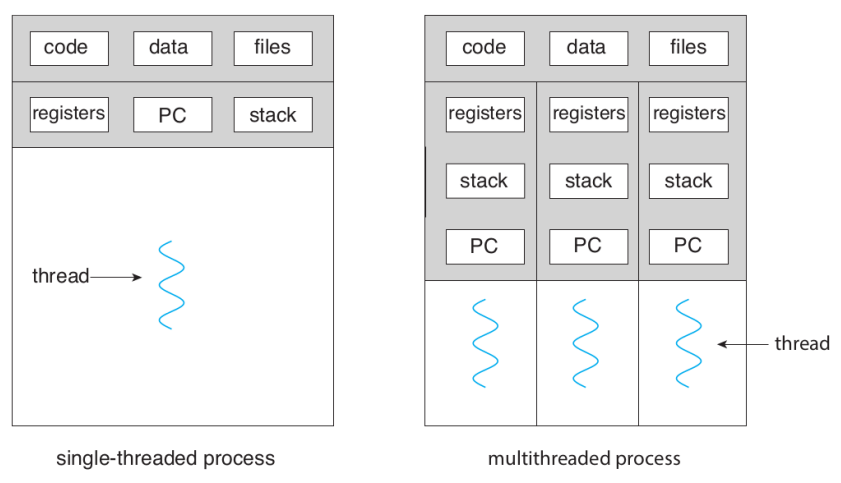
\includegraphics[width=\textwidth]{img/monomulti.png}
\end{figure}

\noindent Hoy en dia, muchos procesos comprenden las multihebras, algunos ejemplos son:
\begin{itemize}
    \item Aplicación para crear imágenes miniatura (thumbnail) desde una colección de imágenes.
    \item Un navegador web puede tener una hebra para la interfaz gráfica y otra para la descarga de archivos.
    \item Un procesador de texto puede tener una hebra enfocada en mostrar gráficos mientras otra se encarga en recibir lo digitado por el usuario y otra para verificar la ortografía.
\end{itemize}
Con esto en cuenta es posible requerir una sola aplicación para realizar varias tareas similares de manera simultanea.
\begin{itemize}
    \item Un servidor web acepta solicitudes de clientes por paginas web, imágenes, sonido, etc.
    \item Sometido a gran carga puede tener miles de solicitudes concurrentes.
    \item Si proceso tiene sola una hebra, atiende una solicitud por vez.
    \item Si proceso crea otros procesos, fork(), lleva tiempo y hace uso intensivo de recursos.
    \item Si proceso es multihebra, por cada solicitud crea una nueva hebra.
\end{itemize}

\begin{figure}[H]
    \centering
    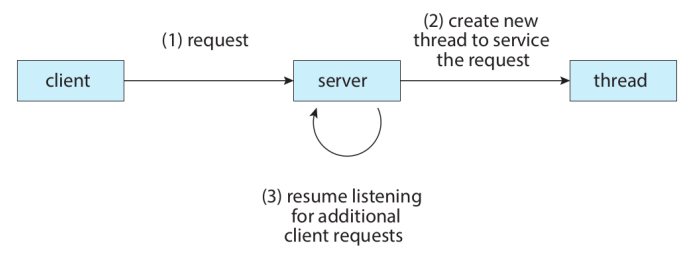
\includegraphics[width=0.5\textwidth]{img/ejemplohebra.png}
\end{figure}

Los SSOO también pueden ser multihebras, por ejemplo Linux al iniciarse crea varias hebras (kernel threads) para tareas especificas como la administración de dispositivos, de memoria, manejo de interrupciones, etc.
Las aplicaciones también se pueden diseñar con este formato para aprovechar las capacidades de los procesadores multihebras. 
\\\\
Algunas de las ventajas de las hebras son: 
\begin{itemize}
    \item \textbf{Capacidad de respuesta}: Si una hebra se bloquea, las demás pueden continuar.
    \item \textbf{Compartición de recursos}: Las hebras comparten recursos del proceso al que pertenecen. Permite a una aplicación tener varias hebras diferentes en un mismo espacio de direcciones.
    \item \textbf{Economía}: Crear una hebra es más económico que crear un proceso tanto en la asignación de recursos como de memoria.
    \item \textbf{Escalabilidad}: Las hebras pueden ser distribuidas en diferentes procesadores, siempre y cuando exista una arquitectura multiprocesador.
\end{itemize}

\subsection*{Programación multinúcleo}
Antes los sistemas operativos eran mononúcleo (single-core), pero hoy en día la mayoría de los sistemas son multinúcleo, por lo que la programacion multihebra proporciona mecanismos para el uso eficiente de estos multiples núcleos.
Si pensamos en una aplicación con cuatro hebras:
\begin{itemize}
    \item En un sistema con un solo núcleo de computación, la concurrencia significa que la ejecución de las hebras se entrelazara en el tiempo.
\end{itemize}
\begin{figure}[H]
    \centering
    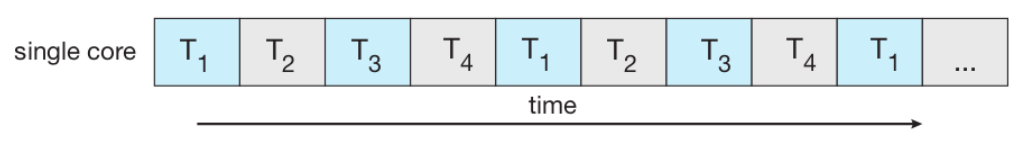
\includegraphics[width=0.8\textwidth]{img/mononucleo.png}
    \caption{Ejecución single-core}
\end{figure}
\begin{itemize}
    \item En un sistema con multiples núcleos, sin embargo, las hebras pueden ejecutarse en paralelo. El sistema puede asignar una hebra a cada núcleo
\end{itemize}
\begin{figure}[H]
    \centering
    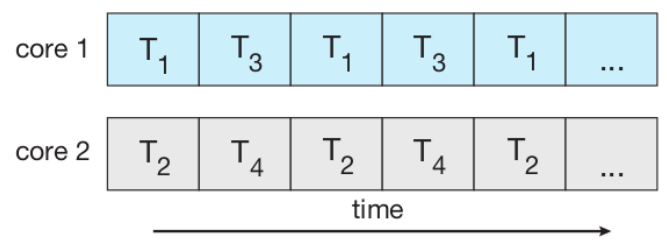
\includegraphics[width=0.5\textwidth]{img/multinucleo.png}
    \caption{Ejecución paralela multi-core}
\end{figure}

\subsection*{Desafíos de la programación multinúcleo}
Al diseñar o modificar programas existentes es necesario tener en cuenta los siguientes desafíos:
\begin{itemize}
    \item Identificación de tareas que puedan ejecutarse idealmente de manera independiente.
    \item Lograr un balance en las cargas de trabajo entre las hebras.
    \item Division de datos para ser usados y manipulados en los diferentes núcleos.
    \item Identificar dependencia de datos que pueden ser accedidos por una o más tareas. 
    \item Sincronización de accesos en los datos compartidos.
    \item Pruebas y depuración aumentan en complejidad.
\end{itemize}

\subsection*{Tipos de paralelismo}
\begin{itemize}
    \item \textbf{Paralelismo de datos}: Se refiere a la distribución de subconjuntos de datos en los multiples núcleos y repetir esto para cada núcleo.
    \item \textbf{Paralelismo de tareas}: Se refiere a la distribución de tareas en los diferentes núcleos.
    \item Se pueden utilizar las 2 técnicas en conjunto ya que no son excluyentes.
\end{itemize}

\begin{figure}[H]
    \centering
    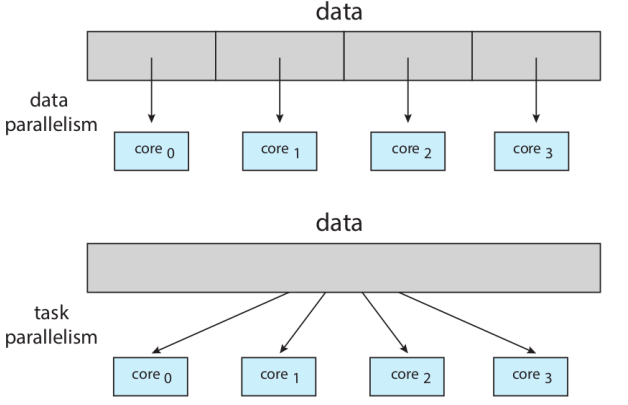
\includegraphics[width=0.7\textwidth]{img/paral.png}
\end{figure}


\subsection*{Modelos multihebra}
En la practica el soporte de hebras puede proporcionarse como:
\begin{enumerate}
    \item \textbf{Hebras de usuario}: Soporte por sobre el kernel, gestión de hebras sin soporte del kernel (POSIX Pthreads, Win32 threads, Java threads).
    \item \textbf{Hebras de kernel}: Kernel soporta y gestiona las hebras (Windows, Linux, macOS).
\end{enumerate}

Debe existir una relación entre las hebras de usuario y las de kernel:
\begin{itemize}
    \item Modelo muchos a uno
    \item Modelo uno a uno
    \item Modelo muchos a muchos
\end{itemize}

\subsubsection*{Modelo muchos a uno}
\begin{itemize}
    \item Cada hebra de usuario es mapeada a una hebra de kernel.
    \item Gestión de hebras en espacio de usuario, mediante una librería.
    \item Proceso completo se bloque si una hebra hace una llamada bloqueante.
    \item Solo una hebra puede acceder al kernel a la vez, no se puede aprovechar el paralelismo.
\end{itemize}

\begin{figure}[H]
    \centering
    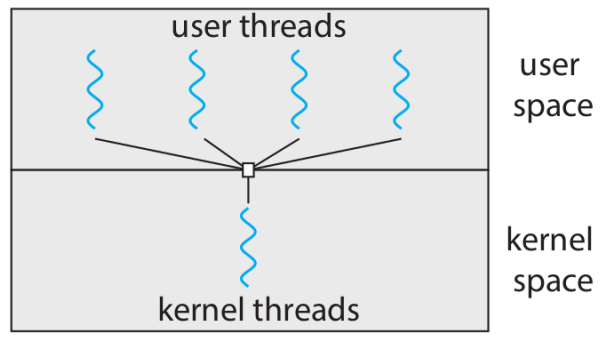
\includegraphics[width=0.5\textwidth]{img/muchos-uno.png}
\end{figure}

\subsubsection*{Modelo uno a uno}
\begin{itemize}
    \item Cada hebra de usuario es mapeada a una hebra de kernel.
    \item Mayor concurrencia que el modelo muchos a uno.
    \item Permite a una hebra bloquearse sin afectar a las demás.
    \item Permite ejecución en varios procesadores.
    \item Se restringe el numero de hebras soportadas por el sistema para no afectar al rendimiento.
    \item Windows, Linux.
\end{itemize}

\begin{figure}[H]
    \centering
    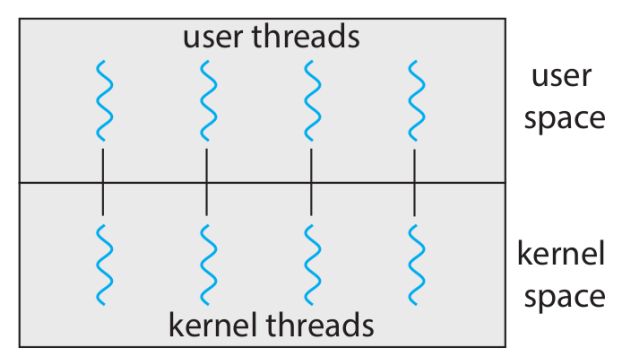
\includegraphics[width=0.5\textwidth]{img/uno-uno.png}
\end{figure}

\subsubsection*{Modelo muchos a muchos}
\begin{itemize}
    \item Asigna muchas hebras de usuario a un numero igual o menor de hebras de kernel.
    \item Se pueden crear tantas hebras de usuario como se desee.
    \item Las hebras de kernel correspondientes se ejecutan en paralelo en un sistema multiprocesador
\end{itemize}

\begin{figure}[H]
    \centering
    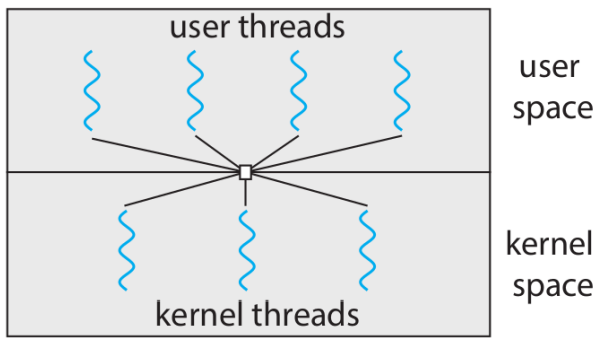
\includegraphics[width=0.5\textwidth]{img/muchos-muchos.png}
\end{figure}

\subsection*{Bibliotecas de hebras}
Son necesarias ya que proporcionan al programador una API para gestionar y crear hebras, existen 2 formas de implementar estas bibliotecas:
\begin{itemize}
    \item Por completo en el espacio de usuario, sin soporte del kernel.
    \begin{itemize}
        \item Estructuras de datos y código de biblioteca en espacio de usuario.
        \item Funciones producen llamadas locales y no al sistema.
    \end{itemize}
    \item Soporte directo del SO
    \begin{itemize}
        \item Estructuras de datos y código de biblioteca en espacio del kernel.
        \item Funciones producen llamadas al sistema.
    \end{itemize}
\end{itemize}
Las 3 principales bibliotecas son:
\begin{itemize}
    \item \textbf{POSIX Pthreads}: API de hebras POSIX, soportada por la mayoría de los sistemas UNIX. Nivel de usuario/kernel.
    \item \textbf{Windows threads}: API de hebras de Windows, soportada por Windows. Nivel de kernel.
    \item \textbf{Java threads API}: API de hebras de Java, soportada por Java. Utiliza librería de hebras existente en el kernel.
\end{itemize}

\subsubsection*{Pthreads}
\begin{itemize}
    \item Basado en el estándar POSIX (IEEE 1003.1c) que define una API para la creación y sincronización de hebras.
    \item Standard UNIX threading API.
    \item Más de 60 funciones: \texttt{pthread\_create}, \texttt{pthread\_join}, \texttt{pthread\_exit}, etc.
    \item Relativamente de bajo nivel.
    \item Manejo explícito de las hebras (creación, eliminación de hebras, sincronización).
    \item Linux, macOS, implementan la especificación Pthreads.
\end{itemize}

\subsubsection*{OpenMP}
\begin{itemize}
    \item Extensión de lenguaje basado en directivas de compilación y biblioteca de funciones.
    \item Disponible para C/C++ y Fortran.
    \item Énfasis en high-performance computing (HPC).
    \item Alto nivel de abstracción.
\end{itemize}

\newpage
\section{Planificación del CPU}
En sistemas con un solo procesador, solo es posible ejecutar un proceso a la vez. Dado que el objetivo de la multiprogramación es maximizar el uso de la CPU, es necesario planificar cuidadosamente la ejecución de los procesos.

En sistemas simples, la CPU queda inactiva mientras espera las operaciones de E/S. Sin embargo, en sistemas más complejos, otros procesos pueden ejecutarse durante ese tiempo de espera.

La ejecución de procesos incluye:
\begin{itemize}
    \item \textbf{Ráfaga de CPU}: Ciclo de ejecución de instrucciones de un proceso.
    \item \textbf{Ráfaga de E/S}: Ciclo de ejecución de instrucciones de un proceso que espera por una operación de E/S.
\end{itemize}

La ejecución de un proceso comienza con una ráfaga de CPU, E/S, etc. La CPU concluye con la solicitud al sistema para finalizar la ejecución.

\begin{figure}[H]
    \centering
    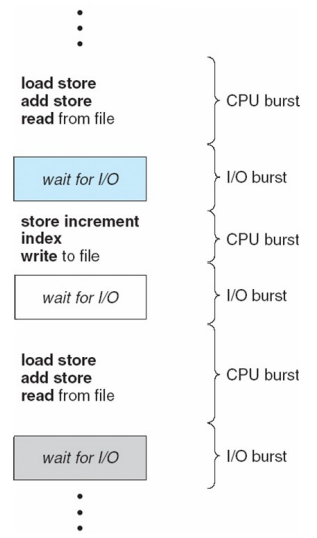
\includegraphics[width=0.35\textwidth]{img/rafagas.png}
    \caption{Ciclos de ráfagas de CPU y E/S}
\end{figure}

\subsection*{Planificador de la CPU}
Recordando los estados de un proceso (ver \hyperref[fig:hormiga-estados]{Hormiga de estados}), observamos las diferentes etapas por las que atraviesa un proceso. El planificador se encarga de seleccionar un proceso de la cola de procesos listos y asignarlo a la CPU.

Esta asignación no necesariamente sigue un formato FIFO, ya que se pueden emplear diferentes algoritmos de planificación, como planificación por prioridad, planificación en árboles, entre otros. Es importante destacar que los elementos en las colas son PCBs (Process Control Blocks), que contienen la información necesaria para gestionar cada proceso (registros).

\subsubsection*{Momento de elección planificación}
La decision de cuando utilizar la planificación es esencial en estas situaciones: 
\begin{enumerate}
    \item Cambio de estado de ejecución (running) a espera (waiting): Solicitud de E/S, espera de un evento, invocación a wait, etc.
    \item Cambia de estado de ejecución (running) a listo (ready): Interrupción de temporizador, fin de la ráfaga de CPU.
    \item Cambia de estado de espera (waiting) a listo (ready): Se completa la operación de E/S.
    \item Termina (terminated)
\end{enumerate}
En planificación \textbf{sin expropiación} el proceso en ejecución no se interrumpe hasta que ocurra 1 o 4 en los cuales entrega la CPU por propia voluntad.
En el resto de los casos se entiende que sucede una planificación \textbf{con expropiación}.


\subsection*{Despachador (Scheduler Dispatch)} 
El despachador es un componente que participa en la planificación de la CPU. Su función es seleccionar un proceso de la cola de procesos listos y asignarlo a la CPU. Dentro de esta función se incluye:
\begin{itemize}
    \item Cambio de contexto: Guardar el estado del proceso que se interrumpe y cargar el estado del proceso que se va a ejecutar.
    \item Cambio de modo usuario: Cambiar de modo kernel a modo usuario.
    \item Salto a posición correcta dentro del programa de usuario para reiniciar la ejecución.
\end{itemize}
Este componente debe ser lo mas rápido posible, ya que el tiempo de cambio de contexto es tiempo muerto y se invoca en cada conmutación de proceso.
La \textbf{latencia de despacho} es el tiempo que tarda en detener un proceso e iniciar otro.


\subsection*{Criterios de planificación}
Dentro de los diferentes algoritmos de planificación existen propiedades que favorecen a una clase de procesos sobre otra. Las propiedades más comunes son:
\begin{itemize}
    \item \textbf{Utilización de la CPU}: Porcentaje de tiempo que la CPU se encuentra ocupada.
    \item \textbf{Tasa de procesamiento - Throughput}: Número de procesos que se completan por unidad de tiempo.
    \item \textbf{Tiempo de ejecución - Turnaround time}: Tiempo transcurrido desde que un proceso entra al sistema hasta que termina (carga de memoria + tiempo de espera + tiempo de ejecución + operaciones de E/S).
    \item \textbf{Tiempo de espera - Waiting time}: Suma de los tiempos que los procesos pasan en la cola de listos.
    \item \textbf{Tiempo de respuesta - Response time}: Tiempo transcurrido desde que se envía una solicitud hasta que se obtiene la primera respuesta.
\end{itemize}

\subsubsection*{Criterios de optimización}
Ya conociendo estas propiedades, se pueden establecer criterios de optimización para los diferentes algoritmos de planificación:
\begin{itemize}
    \item Maximizar la utilización de la CPU.
    \item Maximizar tasa de procesamiento (throughput): Procesar la mayor cantidad de procesos por unidad de tiempo.
    \item Minimizar el tiempo de ejecución (turnaround time): Procesos deben ser completados lo más rápido posible.
    \item Minimizar el tiempo de espera (waiting time): Procesos deben ser atendidos lo más rápido posible.
    \item Minimizar el tiempo de respuesta (response time): Procesos deben ser atendidos lo más rápido posible, especialmente en sistemas de tiempo compartido.
\end{itemize}

\subsection*{Algoritmos de planificación}
Estos algoritmos son la respuesta a la necesidad de optimizar los criterios de planificación. Estos algoritmos puede que resuelvan solo algunos de los criterios de optimización, pero no todos. Algunos de los algoritmos más comunes son:

\subsubsection*{FCFS (First-Come, First-Served)}

Se basa en que el primer proceso que llega es el primero en ser atendido. Es un algoritmo no expropiativo, por lo que el proceso en ejecución no se interrumpe hasta que llega a un estado de espera o termina.

\subsubsection*{SJF (Shortest-Job-First)}

Dentro de los procesos en la lista de listos, se selecciona el proceso con el tiempo de ráfaga de CPU más corto. En el caso de que existan procesos con el mismo tiempo de ráfaga, se selecciona el que llegó primero. A pesar de parecer un buen modelo existe una complicación ya que no siempre se esta seguro del tiempo de ráfaga de CPU.
\\\\
\noindent\underline{\textbf{Propiedades:}}
\begin{itemize}
    \item A cada proceso se le asigna una \textbf{prioridad}.
    \item Proceso con mayor prioridad se le asigna la CPU.
    \item Procesos con la misma prioridad se manejan en \textbf{FCFS}.
    \item Las propiedades pueden ser:
    \begin{itemize}
        \item Apropiativa: Con un procesos en ejecución, se puede cambiar a otro proceso con mayor prioridad.
        \item Cooperativa: Proceso con mayor prioridad se coloca al inicio de la cola.
    \end{itemize}
    \item Problema: \textbf{Inanición} (starvation) - Procesos con baja prioridad pueden no ser atendidos.
    \item Solución: \textbf{Envejecimiento} (aging) - Incrementar la prioridad de los procesos que esperan mucho tiempo.
\end{itemize}

\subsubsection*{Round Robin}
Este algoritmo es un planificador por tiempo, donde cada proceso recibe un tiempo de ejecución fijo, llamado \textbf{quantum} (q = 10 - 100 ms). Si el proceso no ha terminado su ejecución al final del quantum, se coloca al final de la cola de listos y se selecciona el siguiente proceso.
Este quantum debe asignarse de manera que no sea demasiado grande, ya que el algoritmo se convierte en FCFS, y no sea demasiado pequeño, ya que si es menor que el tiempo de cambio de contexto los procesos puede que no se ejecuten.


\subsection*{Colas multinivel} 
Este enfoque clasifica los procesos en grupos distintos, cada uno de los cuales utiliza un algoritmo de planificación específico. Los procesos se organizan en estas colas según sus características o prioridades, permitiendo la aplicación de diferentes estrategias de planificación en cada grupo.
\begin{itemize}
    \item De primer plano (\textbf{foreground}): Se utiliza el algoritmo Round Robin.
    \item De fondo (\textbf{background}): Se utiliza el algoritmo FCFS.
\end{itemize}
Esta diferenciación es aplicada sobre la cola de procesos listos, y como se menciona anteriormente, cada grupo tiene un algoritmo de planificación diferente.


\subsection*{Colas multinivel retroalimentadas}
Este enfoque es similar al de las colas multinivel, pero con la particularidad de que los procesos pueden moverse entre las distintas colas. Si un proceso consume mucho tiempo de CPU, se transfiere a una cola con un quantum más largo. En cambio, si un proceso utiliza poco tiempo de CPU, se desplaza a una cola con un quantum más corto.

La capacidad de moverse entre colas es posible gracias a la retroalimentación que caracteriza a este tipo de planificación. Este mecanismo ayuda a evitar el bloqueo indefinido y la inanición, ya que los procesos que no reciben suficiente tiempo de CPU pueden ser transferidos a una cola con un quantum más adecuado.

\begin{figure}[H]
    \centering
    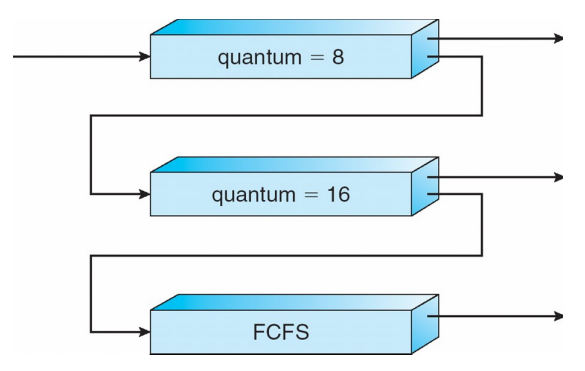
\includegraphics[width=0.45\textwidth]{img/multiniver.png}
    \caption{Ejemplo de colas multinivel retroalimentadas}
\end{figure}

\section{Sincronización de procesos}

El acceder concurrentemente a los datos compartidos puede resultar en datos inconsistentes por lo que mantener datos que sean consistentes requiere de mecanismos para asegurar una ejecución ordenada de procesos cooperativos.

\subsection*{Problema consumidor-productor}

El problema consumidor-productor se basa en que en algún punto de un sistema existen procesos que producen datos y otros que los consumen. El problema radica en que los consumidores no pueden consumir datos que no han sido producidos y los productores no pueden producir datos si no hay espacio para almacenarlos.

\subsection*{Condición de carrera (Race Condition)}

Sucede cuando dos rutinas funcionan correctamente por separado, pero al ejecutarse concurrentemente, el resultado no es el esperado. Esto se debe a que las rutinas comparten recursos y no se han tomado medidas para evitar la interferencia.

\subsection*{Problema de la sección crítica}

La sección crítica es una parte del código donde los procesos acceden a los recursos compartidos (acceso a datos, actualización tablas, etc). Por lo tanto cuando un proceso esta ejecutando su sección crítica, ningún otro proceso debe ser capaz de ejecutar su propia sección crítica.
En un proceso la estructura general es:
\begin{itemize}
    \item Sección de entrada (solicitud para entrar en la sección crítica).
    \item Sección crítica (acceso a los recursos compartidos).
    \item Sección de salida (liberación de los recursos).
    \item Sección restante.
\end{itemize}

El problema de la sección crítica consiste en encontrar un mecanismo que permita a los procesos cooperar sin interferir entre ellos. 

Cualquier solución que se proponga al problema de la sección crítica debe cumplir con los siguientes requisitos:
\begin{enumerate}
    \item Exclusion mutua: Solo un proceso puede ejecutar su sección crítica a la vez.
    \item Progreso: Si ningún proceso está ejecutando su sección crítica y hay procesos que desean entrar en su sección crítica, solo los procesos que no están en su sección crítica pueden decidir quién entra. Esta decisión no puede posponerse indefinidamente.
    \item Espera limitada: Si un proceso desea entrar en su sección crítica, debe ser capaz de hacerlo eventualmente.
\end{enumerate}

Los procesos en modo kernel pueden estar sujetos a posibles condiciones de carrera.

\subsubsection*{Métodos para gestionar la sección critica en SSOO}

\begin{itemize}
    \item \textbf{Kernel apropiativos}
    \begin{itemize}
        \item Proceso puede desalojarse cuando se ejecuta en modo kernel.
        \item Difícil de implementar en arquitecturas SMP.
        \item Versiones comerciales de UNIX (Solaris, IRIX).
        \item Linux V2.6.
        \item Windows 7, 10.
    \end{itemize}
    \item \textbf{Kernel no apropiativos}
    \begin{itemize}
        \item Proceso en modo kernel no se desaloja, se ejecuta hasta que salga del modo kernel, termine, se bloquee o ceda la CPU voluntariamente.
        \item Libre de condiciones de carrera, solo permite un proceso en modo kernel.
        \item Anteriores a Windows 95, kernel tradicional de UNIX y Linux hasta V2.6.
    \end{itemize}
\end{itemize}

\subsubsection*{Soluciones al problema de la sección crítica}

Dentro de la gama de soluciones, el elemento principal que han de tener es la implementación de un \textbf{cerrojo}, el cual evita que las condiciones de carrera se produzcan protegiendo las secciones críticas de los procesos.
Este cerrojo es un hardware de sincronización el cual se caracteriza por:
\begin{itemize}
    \item Ser un soporte de HW para las secciones criticas.
    \item En las maquinas monoprocesadores deshabilitan las interrupciones.
    \item La ejecución del código debe ser sin apropiación.
    \item La instrucción \texttt{test\_and\_set()} es la más utilizada. Sirve para leer y modificar atomicamente una variable. Es una instrucción que no puede ser interrumpida.
    \item Implementarlo en un sistema multiprocesador es más complicado.
\end{itemize}

\subsection*{Sincronización en Linux con Pthreads}

Esta API proporciona cerrojos \textbf{mutex}, variables de condición y cerrojos de lectura/escritura para sincronizar las hebras.

\begin{itemize}
    \item \texttt{\#include \textless{}pthread.h\textgreater{}}
    \item \texttt{pthread\_mutex\_t mutex;}
    \item \texttt{pthread\_mutex\_init(\&mutex, NULL);}
    \item \texttt{pthread\_mutex\_lock(\&mutex);}
    \item \texttt{pthread\_mutex\_unlock(\&mutex);}
\end{itemize}

\subsection*{Sincronización en Linux con clase threads (C++11)}

Esta API no proporciona cerrojos pero si variables de condición para sincronizar las hebras. Los cerrojos se pueden utilizar con otra API.

\begin{itemize}
    \item \texttt{\#include \textless{}mutex\textgreater{}}
    \item \texttt{\#include \textless{}thread\textgreater{}}
    \item \texttt{std::mutex mutex;}
    \item \texttt{mutex.lock();}
    \item \texttt{mutex.unlock();}
\end{itemize}

\newpage
\section{Bloqueos mutuos}

En entornos multiprogramación varios procesos compiten por una cantidad limitada de recursos, por lo tanto el orden en que se van consumiendo los recursos puede afectar el rendimiento del sistema. 
Un bloqueo mutuo (deadlock) es una situación en la que dos o más procesos no pueden continuar ejecutándose porque cada uno de ellos espera un recurso que posee otro proceso.


\subsection*{Modelo del sistema}
Como ya se menciono en estos entornos los recursos escasos son distribuidos entre los \textbf{procesos competitivos}. Estos recursos se clasifican por tipos pudiendo ser ciclos de CPU, espacio de memoria, impresoras, etc. El protocolo de acceso a los recursos para los procesos se basa en la siguiente secuencia:  
\begin{enumerate}
    \item \textit{\textbf{Solicitar recurso}}: Si el recurso esta disponible, se asigna al proceso, si no se bloquea.
    \item \textit{\textbf{Usar el recurso}}: El proceso puede utilizar el recurso asignado.
    \item \textit{\textbf{Liberar recurso}}: Una vez que el proceso ha terminado de utilizar el recurso, lo libera.
\end{enumerate}

\subsection*{Condiciones para el bloqueo mutuo}
Una situación de deadlock se produce cuando se cumplen las siguientes condiciones \textbf{simultáneamente}:
\begin{itemize}
    \item \textbf{Exclusion mutua}: Debe haber a lo menos un recurso que solo pueda ser utilizado por un proceso a la vez (modo exclusivo).
    \item \textbf{Retención y espera}: Un proceso que ya tiene un recurso puede solicitar otro recurso y esperar a que se libere.
    \item \textbf{Sin desalojo}: Los recursos asignados a un proceso no pueden ser desalojados.
    \item \textbf{Esperar circular}: Dos o más procesos están esperando a que se libere un recurso que posee otro proceso.
\end{itemize}

\subsection*{Grafos de asignación de recursos}
Para describir una situación de deadlock se puede utilizar un \textbf{grafo de asignación de recursos}, el cual se compone de:
\begin{itemize}
    \item Vertices (2 tipos):
    \begin{itemize}
        \item Procesos (P): {$P_1, P_2, ... , P_n$} Representados por un círculo.
        \item Recursos (R): {$R_1, R_2, ... , R_m$} Representados por un cuadrado.
    \end{itemize}
    \item Aristas (2 tipos):
    \begin{itemize}
        \item $P_{i} \rightarrow R_{j}$: Asignación de recurso $R_{j}$ al proceso $P_{i}$, arista de solicitud.
        \item $R_{j} \rightarrow P_{i}$: Proceso $P_{i}$ esta esperando el recurso $R_{j}$, arista de asignación.
    \end{itemize}
\end{itemize} 

\begin{figure}[H]
    \centering
    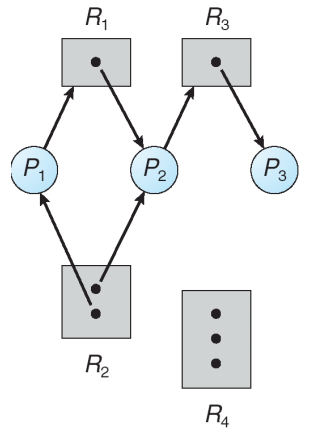
\includegraphics[width=0.5\textwidth]{img/grafo1.png}
    
    $P = \{P_1 , P_2 , P_3\}$\\
    $R = \{R_1 , R_2 , R_3 , R_4\}$\\
    \{$ P_1 \rightarrow R_1 , P_2 \rightarrow R_3 , R_1 \rightarrow P_2 , R_2 \rightarrow P_1 , R_2 \rightarrow P_2 , R_3 \rightarrow P_3 $\}\\
    Instancias: \#$R_1 = 1,$ \#$R_2 = 2$, \#$R_3 = 1$, \#$R_4 = 3$
\end{figure}

\subsubsection*{Condiciones de deadlock}
\begin{itemize}
    \item \textbf{Ciclo en el grafo}(condición necesaria): Si se encuentra un ciclo en el grafo, entonces es posible que exista un deadlock.
    \item \textbf{Ciclo y Recursos}(condición necesaria y suficiente): Si existe un ciclo en el grafo y todos los recursos tienen solo una instancia, entonces es seguro que existe un deadlock.
\end{itemize}
Para los casos en los que no exista ciclos en los grafos, \textbf{no existe deadlock}.

\subsection*{Métodos de manejo de deadlock}
\begin{itemize}
    \item Ignorar el problema y esperar que no ocurra.
    \item Protocolos que aseguran la no ocurrencia de deadlock.
    \begin{itemize}
        \item \textbf{Prevención de deadlock}: Evitar que se cumplan las condiciones necesarias para que ocurra un deadlock.
        \item \textbf{Evitación de deadlock}: Conociendo las necesidades de recurso de los procesos, se analiza la situación para saber si conduce a un deadlock.
    \end{itemize}
    \item Protocolos que aceptan la ocurrencia de deadlock.
    \begin{itemize}
        \item \textbf{Detección y recuperación de deadlock}: Detectar la ocurrencia de un deadlock y recuperarse de él.
    \end{itemize}
\end{itemize}

\subsubsection*{Prevención de deadlock}
Este método se basa en la prevención de la ocurrencia de deadlock, evitando que se cumplan las condiciones necesarias para que ocurra. Estas negaciones serian:
\begin{itemize}
    \item \textbf{Negación de exclusión mutua}: Normalmente es una propiedad del recurso por lo que no es posible obligar a compartir un recurso que no puede ser utilizado de manera simultanea
    \begin{itemize}
        \item \underline{\textbf{Evaluación}}: La exclusión mutua es una propiedad del recurso por lo tanto \textbf{no se puede negar}.
    \end{itemize}
    \item \textbf{Negación de retención y espera}: Un proceso que solicita un recurso no pueda mantener los que ya posee. Lo que se busca es que un proceso solicite todos los recursos que necesita al inicio.
    \begin{itemize}
        \item \underline{\textbf{Evaluación}}: Se pueden asignar recursos pero que no se utilize por periodos de tiempo prolongados. Puede producir postergación indefinida de asignación de recursos.
    \end{itemize}
    \item \textbf{Negación de NO desalojo}: Cuando un recurso que retiene recursos solicita otros, se le pueden desalojar los recursos que ya posee, sin embargo esto provoca que el proceso recomience cuando estén disponibles todos los recursos que necesita.
    \begin{itemize}
        \item \underline{\textbf{Evaluación}}: Esto produce una perdida de trabajo, ademas de causar posiblemente una postergación indefinida y existen recursos que no se pueden expropiar.
    \end{itemize}
    \item \textbf{Negación de espera circular}: Asignación de números a recursos para saber si uno precede a otro, por lo que si un proceso con un recurso de menor número solicita uno de mayor número, se le niega el acceso ya que primero debe liberar el recurso de menor número.
    \begin{itemize}
        \item \underline{\textbf{Evaluación}}: Es difícil asignar un orden a los recurso en un ambiente dinámico, es bastante restrictivo y poco flexible.
    \end{itemize} 
\end{itemize}

\subsubsection*{Evitación de deadlock}
Para evitar la ocurrencia de deadlock se necesita conocer las necesidades de recursos de los procesos, con estos datos se puede realizar asignaciones cuidadosamente.
Esto lograría una mejor utilización de los recursos que la estrategia de prevención, sin embargo, estos métodos mas simples requieren que los procesos conozcan de antemano los recursos máximos que necesitaran.

\begin{itemize}
    \item \textbf{Estado seguro}: Es un estado en el que es posible asignar recursos a los procesos de manera que no se produzca un deadlock.
    \begin{itemize}
        \item Un sistema esta en un estado seguro si existe una secuencia de asignaciones de recursos que permiten a todos los procesos terminar.
        \item Si no existe una secuencia de asignaciones de recursos que permitan a todos los procesos terminar, el sistema esta en un estado inseguro.
        \item Un estado seguro evita la ocurrencia de deadlock.
        \item Un estado inseguro no garantiza un deadlock pero puede conducir a uno.
    \end{itemize}
\end{itemize}
\begin{figure}[H]
    \centering
    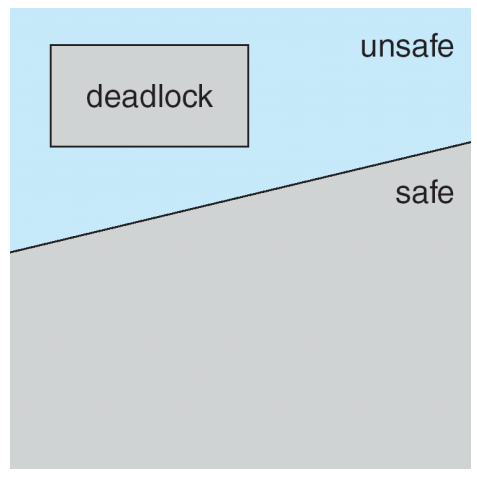
\includegraphics[width=0.4\textwidth]{img/estadoSeguro.png}
\end{figure}


\subsubsection*{Evitación de deadlock - Algoritmo del banquero (Dijkstra 1965)}
Se basa en que un proceso solicita recursos y el sistema verifica si la asignación de recursos puede llevar a un estado seguro. Si es así, se asignan los recursos, si no, el proceso debe esperar. Para ello se requiere que cuando una nueva hebra entre al sistema declare el máximo número de recursos que necesitará.

\subsection*{Detección y recuperación de deadlock}
Mediante un algoritmo se detecta si existe un deadlock, este algoritmo permite la existencia de las 3 primeras condiciones para la ocurrencia de un deadlock y detecta la cuarta.

\newpage
\begin{itemize}
    \item \textbf{Idea}
    \begin{itemize}
        \item El SO chequea periódicamente si hay un ciclo en el grafo de asignación de recursos y si lo hay, si detecta un deadlock.
        \item En caso de detectar un deadlock, el SO puede inicia un procedimiento de recuperación.
    \end{itemize}
\end{itemize}
Cuando el algoritmo detecta la existencia de una deadlock puede tomar una de las siguientes acciones:
\begin{itemize}
    \item \textbf{Recuperación manual}: Avisar al usuario de la existencia de un deadlock y que este tome las medidas necesarias.
    \item \textbf{Recuperación automática}: El SO toma las medidas necesarias para recuperarse del deadlock mediante:
    \begin{itemize}
        \item Abortar uno o más procesos.
        \item Expropiación de uno o más recursos.
    \end{itemize}
\end{itemize}


\subsubsection*{Abortar uno o más procesos}
\begin{itemize}
    \item \textbf{Técnicas}
    \begin{itemize}
        \item Abortar todos los procesos bloqueados.
        \item Abortar los procesos bloqueados de a uno e ir viendo si se termino el deadlock.
    \end{itemize}
    \item \textbf{Criterios}
    \begin{itemize}
        \item Prioridad del proceso.
        \item Tiempo de ejecución que lleva el proceso.
        \item Cantidad y tipo de recursos que posee el proceso.
        \item etc.
    \end{itemize} 
\end{itemize}

\subsubsection*{Expropiación de uno o más recursos}
Consiste en quitar sucesivamente los recursos a los procesos y asignárselos a otros hasta romper el ciclo de bloqueo. Se debe considerar:
\begin{itemize}
    \item Selección de victima: Intentar elegir el proceso que minimice el costo de la expropiación.
    \item Rollback (vuelta atrás): Si se expropia un recurso a un proceso, este debe volver a un punto de seguridad (estado anterior).
    \item Inanición: Asegurarse que el proceso al que se le expropian recursos no sea el mismo siempre.
\end{itemize}

\newpage
\section{Memoria principal (MP)}

\subsection{Fundamentos}
Para entender la gestión de la memoria principal es necesario conocer los siguientes conceptos:
\begin{itemize}
    \item Los programas deben estar cargados en MP para ser ejecutados.
    \item La MP y los registros integrados del procesador son las únicas áreas de almacenamiento al que la CPU puede acceder directamente.
    \item La MP es un arreglo de bytes identificados por direcciones únicas.
    \item La interacción con la MP se logra mediante secuencias de lecturas o escrituras de direcciones especificas de la memoria.
    \item El caché es la memoria más rápida entre la MP y la CPU y se utiliza para resolver problemas de velocidades.
    \item Se requiere garantizar la correcta operación que proteja al SO y los procesos de usuarios de accesos indebidos (registros base y limite). 
\end{itemize}

\subsection{Registros base y límite}
El par de registros base y limite \textbf{definen el espacio de direcciones para cada proceso}. De manera mas especifica el registro base \textbf{almacena la dirección de memoria física legal mas pequeña}, mientras que el registro limite  \textbf{especifica el tamaño del rango}.

La protección de espacio realizada por estos registros se logra haciendo que el HW de la CPU compare las direcciones generadas modo usuario con el contenido de estos registros.

Cualquier acceso ilegal (fuera del rango) provoca una interrupción hacia el SO.

\begin{figure}[H]
    \centering
    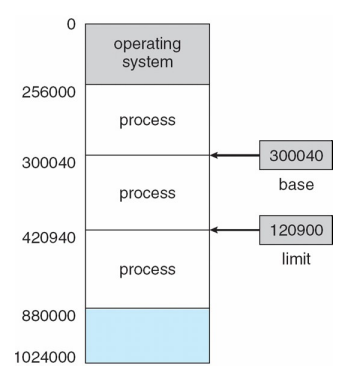
\includegraphics[width=0.45\textwidth]{img/baseylimite.png}
\end{figure}

\subsection{Reasignación de direcciones}
Es necesario que los programas de usuario recorran varias etapas antes de ser ejecutados, donde las direcciones pueden representarse de diferentes formas.
\begin{itemize}
    \item Programa fuente, las direcciones son simbólicas (la variable "suma").
    \item Luego, el compilador reasignará tal dirección simbólica a reubicables (14 bytes a partir de este modulo).
    \item El cargador reasignará la dirección reubicable a direcciones absolutas (74014).
\end{itemize}
\textbf{Cada operación de Reasignación constituye una relación de un espacio de direcciones a otro}.

La Reasignación de direcciones se puede realizar en cualquiera de estas etapas:
\begin{itemize}
    \item \textbf{Tiempo de compilación}: Si se conoce donde va a residir el proceso al momento de compilar, el compilador puede generar un \textbf{código absoluto}. Si se cambia la ubicación, se hace necesario recompilar el programa (programas .COM de MS-DOS).
    \item \textbf{Tiempo de carga}: Si no se conoce la ubicación del proceso al momento de compilar, se genera un \textbf{código reubicable}. La Reasignación final se ralentiza hasta el momento de la carga. Luego si cambia la ubicación, solo es necesario cargar el código del usuario.
    \item \textbf{Tiempo de ejecución}: Si el proceso puede moverse durante su ejecución desde un segmento de memoria a otro, se retarda la Reasignación final hasta el instante de la ejecución. Requiere de un HW especial (MMU - Memory Management Unit). La memoria de los SSOO de propósito general utilizan este método.
\end{itemize}

\subsection{Etapas para la ejecución de un programa}
\begin{figure}[H]
    \centering
    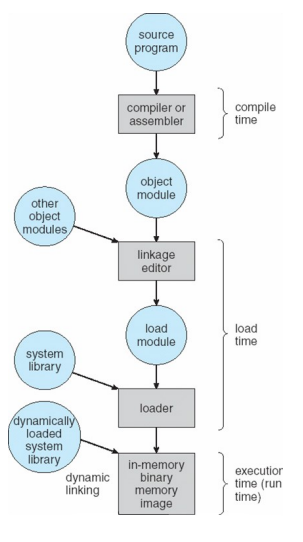
\includegraphics[width=0.325\textwidth]{img/cargaprograma.png}
\end{figure}

\subsection{Espacio de direcciones lógicas y físicas}
\begin{itemize}
    \item \textbf{Dirección lógica}: Dirección generada por la CPU, vista por el proceso.
    \item \textbf{Dirección física}: Dirección recibida por la unidad de memoria y que puede ser eventualmente distinta a la dirección lógica.
    \item \textbf{Espacio de direcciones lógicas}
    \item \textbf{Espacio de direcciones físicas}
\end{itemize}





\end{document}
